\chapter{Design and Implementation}

\section{OTA Design}
The first stage of the design is the Operational Transconductance Amplifier. This stage uses bipolar power supply of 2.5V and -2.5V. Two separate designs - OTA with PMOS Differential pair and OTA with NMOS Differential pair were deisgned and simulated in Cadence to get a good understanding of the circuit parameters and how the differential pair impact them. 

Generally, amplifiers with PMOS transistors used as differential input offer high linearity, low flicker (1/f) noise. A possible reason to choose PMOS transistors as a differential pair comes from the necessity to reduce the influence of the substrate noise. The two transistors are in an N-well and the well is connected to the supply voltage that any substrate interference coupled via the parasitic capacitance to substrate is decoupled to the VDD line. P-channels typically have less flicker noise (1/f noise) caused by the carriers randomly enterring and leaving traps introduced by defects near the semiconductor surface. Since the majority charge carriers are holes in PMOS, there are less potential to be trapped in surface states.

Having stated all these facts, NMOS input transistors would be better in terms of transconductance gain, and hence thermal noise and the bandwidth of the amplifier. An important fact considered in the selection of the type of differential pair is that the OTA in this system is being used in an open loop. This means that the gain of the OTA has to be limited in order to avoid saturation at the crests and troughs at the output of the OTA.

PMOS transistors exhibit their low noise behaviour due to the fact that PMOS transistors are usually bigger (higher W/L ratio) than an NMOS pair. Since we need a small open loop gain, we cannot afford to have big transistors at the input that cause the output to saturate. Along with this, it was also seen that, the range of bias currents needed to obtain a similar range of voltage swing was much wider in case of PMOS than NMOS. Since this indirectly results in a high power dissipation in the 1st stage itself, it was concluded to use the NMOS based design as part of this Thesis work.

\subsection{Schematic}

Figure.\ref{fig:OTA_Schematic} shows the schematic of the OTA used as part of this Thesis. As mentioned above, the differential amplifier is formed by the NMOS pair. The bias current $I_{bias}$ to the differential pair is provided by the current mirror formed by $M_{nB1}$ and $M_{nB2}$ which is in turn controlled by the PMOS transistor $M_9$ whose gate voltage $V_{bias}$ is the programmable variable of the OTA and the entire system. This bias voltage is inversely proportional to the bias current flowing through each branch of the OTA.

\begin{figure} [H]
\centering
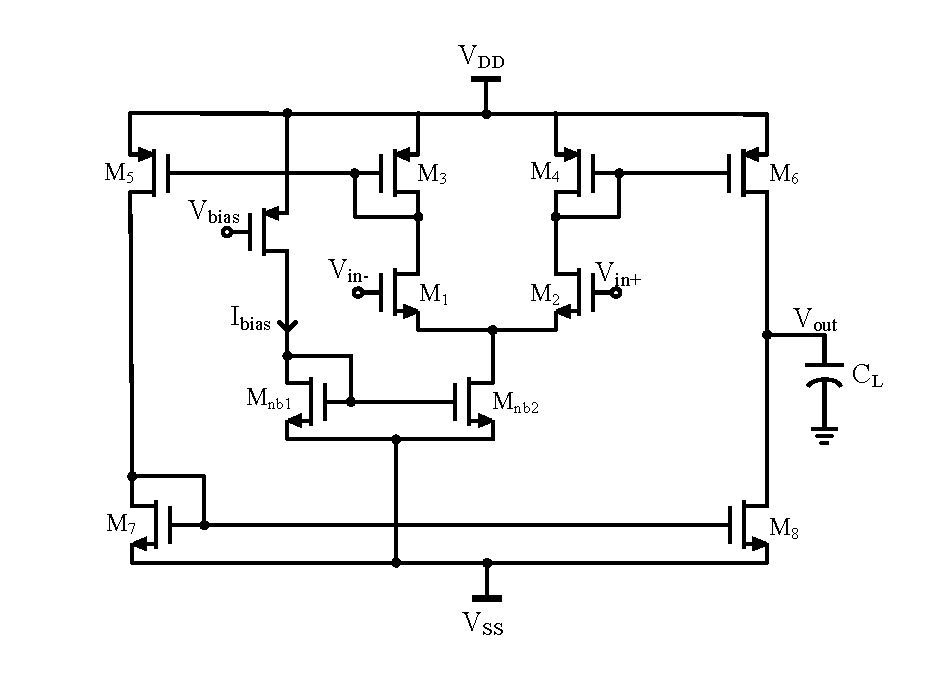
\includegraphics[scale=1]{Figures/Schematics/OTA_NMOS_Vbias.pdf}
\caption{Schematic of the OTA Designed}
\label{fig:OTA_Schematic}
\end{figure}

\begin{table} [H]
\centering
\begin{tabular}{@{}cccc@{}}
\toprule
Transistor			& Width				& Length			& Multiplier \\ \midrule
M1					& 8u				& 500n				& 5			\\
M2					& 8u				& 500n				& 5			\\
M3					& 35u				& 500n				& 1			\\
M4					& 35u				& 500n				& 1			\\
M5					& 28u				& 500n				& 3			\\
M6					& 35u				& 500n				& 3			\\
M7					& 35u				& 500n				& 18		\\
M8					& 33u				& 500n				& 18		\\
M9					& 10u				& 500n				& 4			\\
MnB1				& 20u				& 500n				& 8			\\
MnB2				& 20u				& 500n				& 8			\\
\bottomrule
\end{tabular}
\caption{Dimensions of the Transistors of the designed OTA}
\label{tab:OTA_dimensions}
\end{table}


From the Table.\ref{tab:OTA_dimensions}, it can be seen that the current mirror gain for the current mirrors formed by $M_{3}$, $M_{5}$ and $M_{4}$, $M_{6}$ is 3. It can also be noted that the transistors $M_{5}$ and $M_{8}$ are not symmetric with respect to their counterparts. This is designed so to make sure the DC bias point at the output of the OTA is close to 0V, which is the mid point of $V_{DD}$ and $V_{SS}$. Changing the bias current of an amplifier, will automatically change the DC bias point at its output. Since we are using the OTA as a programmable block, it is important to have an output which is symmetric over 0. Even though it is not entirely possible, making these two transistors a little assymetric or uneven would close the gap between the bias points for highest and lowest bias currents.

\subsection{Test Setup}

In the following subsections, let us look at how this $V_{bias}$ affects various paramters of the OTA by performing DC, AC, Transient and Noise Analyses.

\subsubsection{DC Analysis}

The circuit in Figure.\ref{fig:OTA_TB_ACDC}, is a common test bench  to measure various parameters. The AC source in $V_{ac}$ does not impact the DC analysis in any way. So for the DC analysis, the differential pair transistors will have a voltage of $V_{cm}$ at its gates. $V_{bias}$ is the variable supply used as a programmable parameter and a capacitive load to measure the outputs.

$V_{DD}$ = 2.5V; $V_{SS}$ = -2.5V; $V_{cm}$ = 1.95V; $V_{bias}$ = 150mV to 700mV;  $V_{ac}$ = 1V; $C_{L}$ = 50fF.

\begin{figure} [H]
\centering
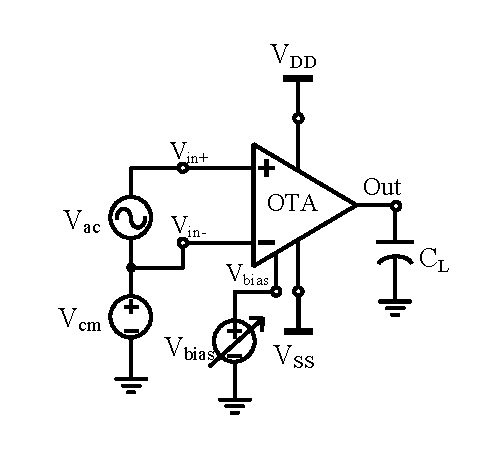
\includegraphics[scale=1]{Figures/Test_Benches/OTA/OTA_ACDC.pdf}
\caption{OTA Test setup for AC, DC and Noise Analysis}
\label{fig:OTA_TB_ACDC}
\end{figure}

\begin{table} [H]
\centering
\begin{tabular}{@{}cccccccc@{}}
\toprule
Vbias (mV)					& 150		& 200			& 300			& 400			& 500			& 600			& 700 \\ \midrule
Output DC Bias (mV)			& 13.68		& -16.43		& -78.96		& -144.6		& -213.3		& -285.2		& -360.3 \\
\bottomrule
\end{tabular}
\caption{Output DC Bias Point of the OTA}
\label{tab:OTA_DC_Bias}
\end{table}

The output DC bias points for various values of $V_{bias}$ is tabulated in Table\ref{tab:OTA_DC_Bias}. The DC voltage at the output decreses with the increase in bias voltage or decrease in bias current.

\subsubsection{AC Analysis}
Figure. \ref{fig:OTA_TB_ACDC} is used for AC analysis as well. \\
$V_{DD}$ = 2.5V; $V_{SS}$ = -2.5V; $V_{cm}$ = 1.95V; $V_{bias}$ = 150mV to 700mV;  $V_{ac}$ = 1V; $C_{L}$ = 50fF.

The same parameters hold good for AC analysis as well. Here, the value of $V_{ac}$ becomes significant. The value of the open loop gain is given by the ratio of output voltage to input voltage.

Gain = $\frac{V_{out}}{V_{in}}$\\
Gain in dB = $20 log_{10}\frac{V_{out}}{V_{in}}$

Figure\ref{fig:OTA_Gain} shows the semilog plot of Gain for maximum and minimum $V_{bias}$. The plots for the other values of $V_{bias}$ are not shown here as that would make the plot less legible for understanding and more so because those plots would be in between the plots already shown.

\begin{figure} [H]
\centering
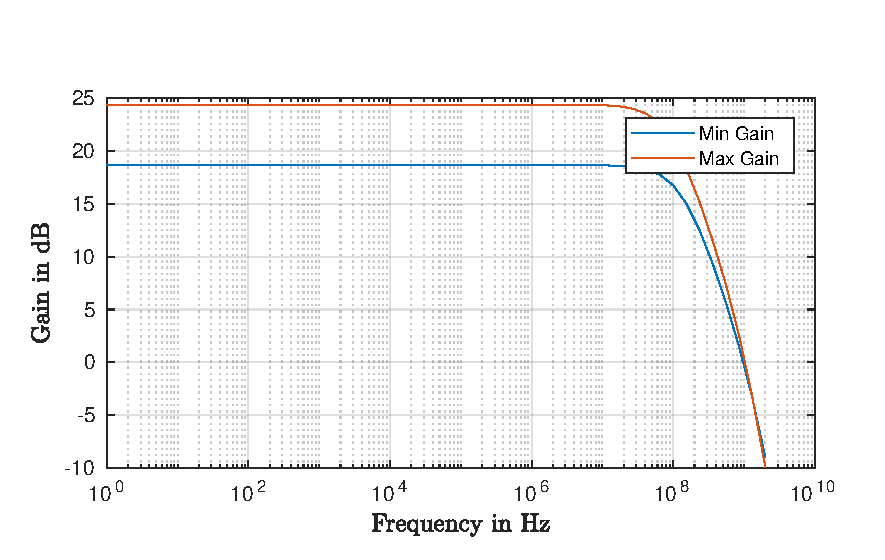
\includegraphics[scale=1]{Figures/Plots/OTA_Gain.pdf}
\caption{OTA Plot of Gain vs Frequency for different Vbias}
\label{fig:OTA_Gain}
\end{figure}

The variation of open loop gain of the OTA, its bandwidth and the phase margin with respect to $V_{bias}$ is tabulated in Table.\ref{tab:OTA_gain_bw_pm}. The bandwidth is kept at a high value in order to make sure that the dominant poles of the first and second stages are sufficiently far from each other so as to obtain a stable system for operation. The maximum open loop gain for this system is 23.7dB. Any value beyond this will cause the amplifier to saturate at the crests and troughs of the output voltage.

\begin{table} [H]
\centering
\begin{tabular}{@{}cccccccc@{}}
\toprule
Vbias (mV)					& 150		& 200		& 300		& 400		& 500		& 600		& 700 \\ \midrule
Open Loop Gain (dB)			& 18.64		& 19.46		& 20.9		& 22.05		& 22.96		& 23.7		& 24.35 \\
Phase Margin (degrees)		& 63.3		& 60.63		& 55.96		& 52.42		& 49.91		& 48.12		& 46.72 \\
Bandwidth (MHz)				& 135		& 130.7		& 122.2		& 113.7		& 105		& 96.63		& 89.19 \\
\bottomrule
\label{tab:OTA_gain_bw_pm}
\end{tabular}
\caption{Open Loop Gain, Phase Margin and Bandwidth of the OTA}
\end{table}

\begin{figure} [H]
\centering
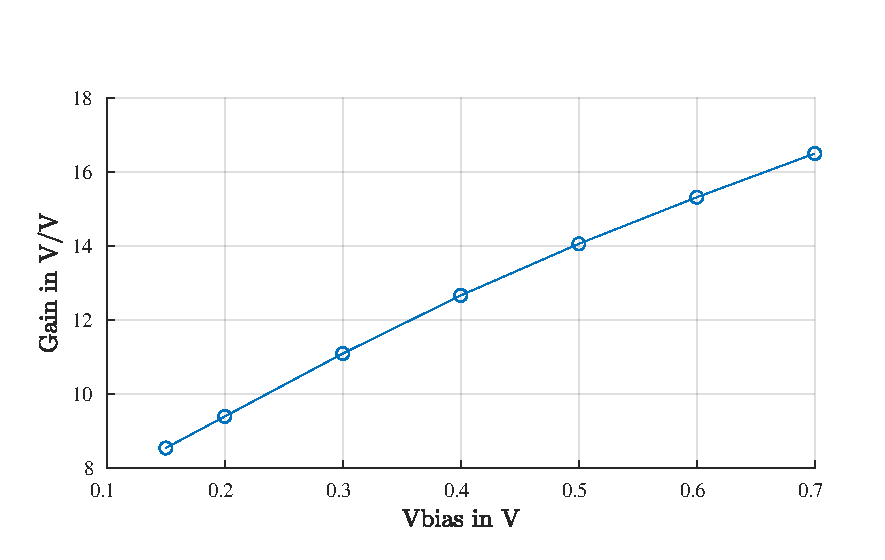
\includegraphics[scale=1]{Figures/Plots/OTA_Gain_Abs.pdf}
\caption{OTA Plot of Gain vs Vbias}
\label{fig:OTA_gain_abs}
\end{figure}

On the same lines, the variation of absolute value of gain with respect to different values of $V_{bias}$ is seen in Figure\ref{fig:OTA_gain_abs} tabulated in Table.\ref{tab:OTA_gain_abs}. The reason to choose the values of $V_{bias}$ are evident from this table and that is because it provides us a gain in the ratio of almost 1:2 for those values of $V_{bias}$. As seen from the table of specifications that we need a transconductance in the ratio of 1:1.8 or something close to that.

\begin{table} [H]
\centering
\begin{tabular}{@{}cccccccc@{}}
\toprule
Vbias (mV)					& 150			& 200			& 300			& 400			& 500			& 600			& 700 \\ \midrule
DC Gain (V/V)			& 8.548		& 9.4		& 11.1		& 12.67		& 14.06		& 15.31		& 16.49 \\
\bottomrule
\end{tabular}
\caption{Absolute values of DC Gain of the OTA}
\label{tab:OTA_gain_abs}
\end{table}

\subsubsection{Noise Analysis}

Once again, we use the same test bench as shown in Figure.\ref{fig:OTA_TB_ACDC}. As mentioned in the previous section, the NMOS differential pair exhibits high flicker noise, also known as 1/f noise. This noise is significant at low frequencies. At moderate and high frequencies, the effect of thermal or white noise is much more dominant and hence flicker noise becomes less significant at those frequencies.

The variation of the input referred noise with respect to $V_{bias}$ is tabulated in Table.\ref{tab:OTA_Noise}. With increase in $V_{bias}$, the input referred noise decreases. This is because the gain increases with increase in $V_{bias}$ and consequently input referred noise decreases. This also converges to the fact that the input referred noise decreases with bigger dimensions of the differential pair, and thereby contributing to a higher gain.

\begin{table} [H]
\centering
\begin{tabular}{@{}cccccccc@{}}
\toprule
Vbias (mV)					& 150			& 200			& 300			& 400			& 500			& 600			& 700 \\ \midrule
Input Referred Noise (nV/$\sqrt{Hz}$)			& 46.36		& 43.73		& 39.83		& 37.29		& 35.57		& 34.31		& 33.28 \\
\bottomrule
\end{tabular}
\caption{Input Referred Noise of the OTA}
\label{tab:OTA_Noise}
\end{table}

\subsubsection{Transient Analysis - Sine Input}

The test bench in Figure.\ref{fig:OTA_TB_Sine} is used to measure the transient parameters for a sine wave input. An ideal balun is used at the input to provide a differential voltage to the terminals. The voltages are 180$^0$ out of phase with each other. 

$V_{DD}$ = 2.5V; $V_{SS}$ = -2.5V; $V_{cm}$ = 1.95V; $V_{bias}$ = 150mV to 700mV;  $V_{sin} amplitude$ = 100mV; $frequency = 1MHz$ $C_{L}$ = 50fF.

\begin{figure} [H]
\centering
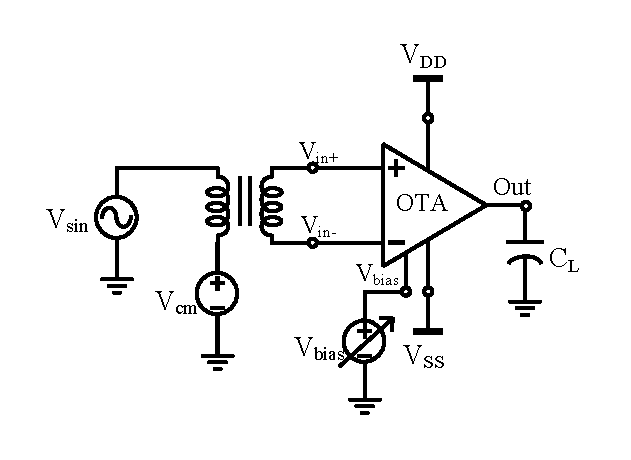
\includegraphics[scale=1]{Figures/Test_Benches/OTA/OTA_Sine.pdf}
\caption{OTA Test setup for Transient Analysis - Sine Wave Input}
\label{fig:OTA_TB_Sine}
\end{figure}

The transient simulation is carried out for 3$\mu $s. The sinusoidal output with respect to time is shown in Figure.\ref{fig:OTA_Sine} for different values of $V_{bias}$. As we know from the AC analysis, the gain varies in the ratio of 1:2 and thereby, here we have the peak-to-peak voltages varying in the same ratio. And as discussed in the DC Analysis, the DC bias points at the output are close to zero but not exactly at 0 for all the $V_{bias}$ values.

\begin{figure} [H]
\centering
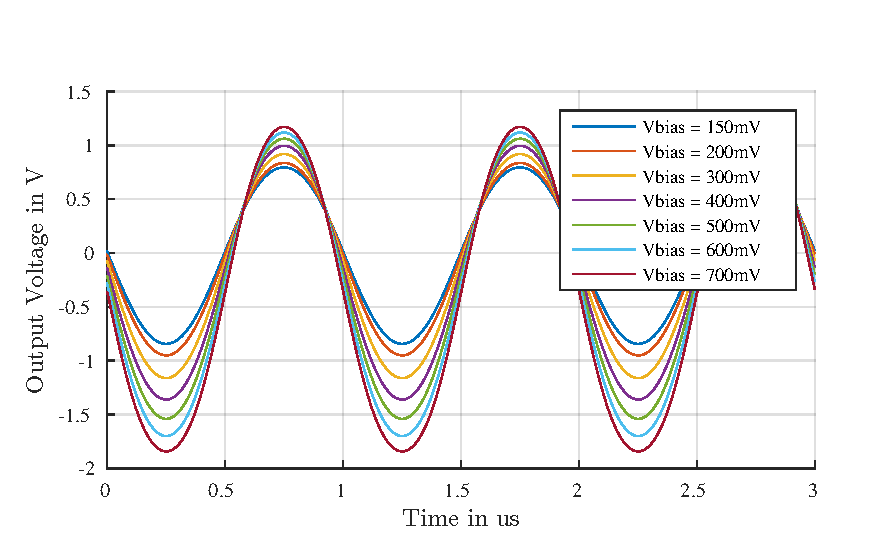
\includegraphics[scale=1]{Figures/Plots/OTA_Sine.pdf}
\caption{OTA Output Voltage for vs time for different Vbias}
\label{fig:OTA_Sine}
\end{figure}

Table\ref{tab:OTA_Sine_Params} shows the variation of different transient parameters with respect to $V_{bias}$. The voltage swing varies from 1.639 to 3.014 which is almost in the ratio of 1:2. HD3 worsens with increase in $V_{bias}$ and on the contrart, improves. Although, it is seen that the HD2 again starts to worsen beyond 600mV of $V_{bias}$.

\begin{table} [H]
\centering
\begin{tabular}{@{}cccccccc@{}}
\toprule
Vbias (mV)					& 150			& 200			& 300			& 400			& 500			& 600			& 700 \\ \midrule
Vout Max (V)			& 0.7949		& 0.8362		& 0.9188		& 0.995		& 1.061		& 1.119		& 1.172 \\
Vout Min (V)			& -0.844		& -0.9505		& -1.162		& -1.361		& -1.54		& -1.7		& -1.842 \\
Vout Swing (V)				& 1.639		& 1.787		& 2.081		& 2.356		& 2.601		& 2.818		& 3.014 \\
HD2 (dBc) 				& -44.83		& -44.28		& -43.86		& -44.74		& -47.97		& -60.86		& -48.75 \\
HD3 (dBc) 				& -52.15		& -49.69		& -46.13		& -43.87		& -42.24		& -40.78		& -39.32 \\
\bottomrule
\end{tabular}
\caption{Transient Parameters of the OTA}
\label{tab:OTA_Sine_Params}
\end{table}

\subsubsection{Transient Analysis - Square Input}
The test bench in Figure.\ref{fig:OTA_TB_Slew} is used to measure the transient parameters for a square wave input. Slew rate is the rate of change of output voltage. It is also defined as the ratio of bias current to load capacitance.

$V_{DD}$ = 2.5V; $V_{SS}$ = -2.5V; $V_{cm}$ = 1.95V; $V_{bias}$ = 150mV to 700mV;  $V_{pulse} V_1$ = 100mV; $V_2$ = -100mV; $Pulse Width$ = 49.7ns; $Period$ = 100ns; $Rise Time$ = 300ps; $Fall time$ = 300ps; $C_{L}$ = 50fF.

\begin{figure} [H]
\centering
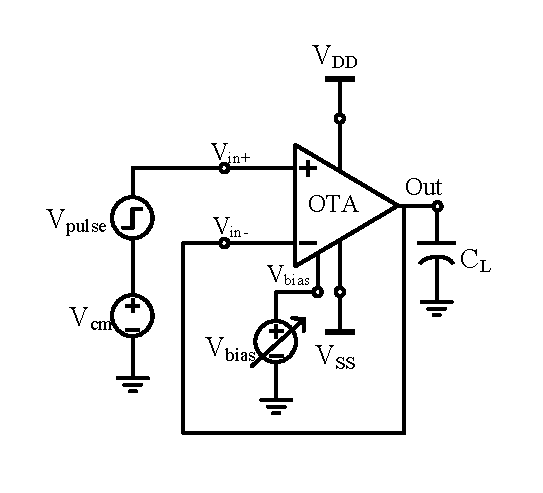
\includegraphics[scale=1]{Figures/Test_Benches/OTA/OTA_Slew.pdf}
\caption{OTA Test setup for Transient Analysis - Square Wave Input}
\label{fig:OTA_TB_Slew}
\end{figure}
The slew rate, both for the rising edge and the falling edge is tabulated in the Table.\ref{tab:OTA_Slew}.

\begin{table} [H]
\centering
\begin{tabular}{@{}cccccccc@{}}
\toprule
Vbias (mV)					& 150			& 200			& 300			& 400			& 500			& 600			& 700 \\ \midrule
Slew Rate Rising Edge (V/us)			& 386.9		& 407.8		& 452.9		& 501.9 	& 547.6		& 585.4		& 609.3 \\
Slew Rate Falling Edge (V/us)			& -389		& -413.8		& -469.4		& -523.5		& -570.5		& -605.7		& -626.4 \\
\bottomrule
\end{tabular}
\caption{Slew Rate of the OTA}
\label{tab:OTA_Slew}
\end{table}

\subsubsection{AC Analysis - PSRR}
PSRR or Power Supply Signal Ratio is defined as the ability of an amplifier to maintain its output as its DC power supply is varied. Is is the ratio of change in the output current to change in power supply.

$ PSRR = \frac{\Delta I_{out}}{\Delta V_{DD}}$

$V_{DD}$ = 2.5V; $AC Magnitude of V_{DD}$ = 1V; $V_{SS}$ = -2.5V; $V_{cm}$ = 1.95V; $V_{bias}$ = 150mV to 700mV; $C_{L}$ = 50fF.
\begin{figure} [H]
\centering
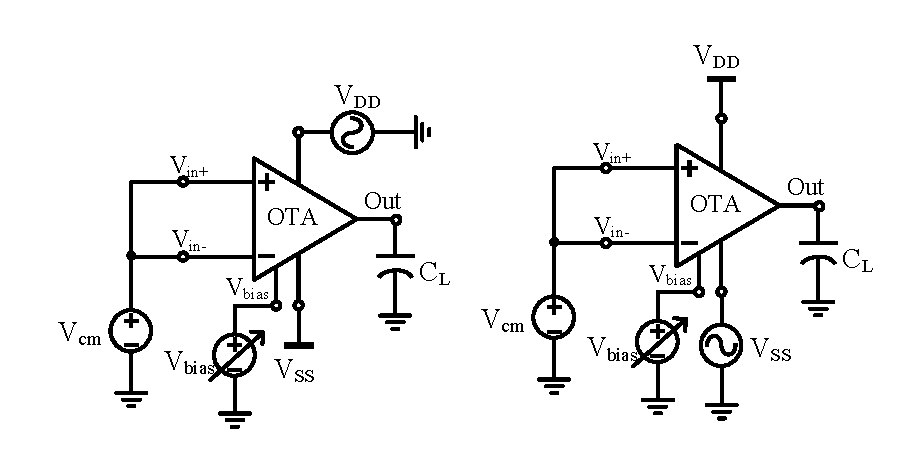
\includegraphics[scale=1]{Figures/Test_Benches/OTA/OTA_PSRR.pdf}
\caption{OTA Test setup for calculating PSRR}
\label{fig:OTA_TB_PSRR}
\end{figure}
$V_{DD}$ = 2.5V; $V_{SS}$ = -2.5V; $AC Magnitude of V_{SS}$ = 1V; $V_{cm}$ = 1.95V; $V_{bias}$ = 150mV to 700mV; $C_{L}$ = 50fF.

The test bench to measure the PSRR of the OTA is as shown in the Figure.\ref{fig:OTA_TB_PSRR}. The one on the left is used to measure PSRR for a change in $V_{DD}$. And similarly, the one on the right side is used to measure PSRR for a change in $V_{SS}$.

The variation of PSRR with respect to $V_{bias}$ is tabulated in Table.\ref{tab:OTA_PSRR}. The PSRR is fairly low in the range of nA/V and increases only slightly with increase in $V_{bias}$.

\begin{table} [H]
\centering
\begin{tabular}{@{}cccccccc@{}}
\toprule
Vbias (mV)					& 150			& 200			& 300			& 400			& 500			& 600			& 700 \\ \midrule
PSRR (VDD Supply) (nA/V)			& 234.6		& 236.9		& 241.6		& 246.7 	& 252.2		& 258		& 264.3 \\
PSRR (VSS Supply) (nA/V)			& 254.5		& 256.5		& 260.4		& 264.2		& 267.9		& 271.5		& 274.9 \\
\bottomrule
\end{tabular}
\caption{Power Supply Rejection Ratio of the OTA}
\label{tab:OTA_PSRR}
\end{table}

\subsubsection{AC Analysis - Input Impedance}
OTAs generally exhibit a very high input impedance. And to measure this parameter, an AC current source with a magnitude of 1A is connected to the non-inverting terminal of the OTA. And the input impedance is given by the ratio of the AC voltage to the AC current at the input of the OTA. Since the current at the input is 1A, the magnitude of the input voltage will be the value of the input impedance in Ohms at that particular frequency. Since the OTA operation is carried out at 1MHz, the voltage at 1MHz is considered to obtain the value of Input Impedance. Figure.\ref{fig:OTA_TB_ZIN} shows the test bench to measure the input impedance.

$V_{DD}$ = 2.5V; $V_{SS}$ = -2.5V; $V_{bias}$ = 150mV to 700mV; $C_{L}$ = 50fF; $I_{sin} magnitude$ = 1A. 

\begin{figure} [H]
\centering
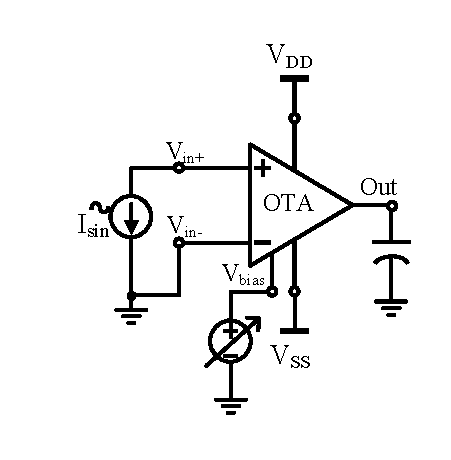
\includegraphics[scale=1]{Figures/Test_Benches/OTA/OTA_Zin.pdf}
\caption{OTA Test setup for calculating Input Impedance}
\label{fig:OTA_TB_ZIN}
\end{figure}

The variation of input impedance with respect to $V_{bias}$ is tabulated in Table.\ref{tab:OTA_ZIN}. The variation is quite small and it increases slightly with an increase in bias voltage and is in the order of Mega Ohms.

\begin{table} [H]
\centering
\begin{tabular}{@{}cccccccc@{}}
\toprule
Vbias (mV)					& 150		& 200			& 300			& 400			& 500			& 600			& 700 \\ \midrule
Input Impedance (M$\Omega$)			& 3.38		& 3.388		& 3.403		& 3.419		& 3.434		& 3.45		& 3.467 \\
\bottomrule
\end{tabular}
\caption{Input Impedance of the OTA}
\label{tab:OTA_ZIN}
\end{table}

\subsubsection{AC Analysis - Output Impedance}

In a concept similar to measuring the input impedance, the output impedance too, is measured with a help of a current source with unity magnitude at the output instead of a Capacitive load. The differential inputs are connected in a common mode configutation. The test bench to measure the output impedance of the OTA is as shown in Figure.\ref{fig:OTA_TB_ZOUT}.

$V_{DD}$ = 2.5V; $V_{SS}$ = -2.5V; $V_{cm}$ = 1.95V $V_{bias}$ = 150mV to 700mV; $I_{sin} magnitude$ = 1A. 
 
\begin{figure} [H]
\centering
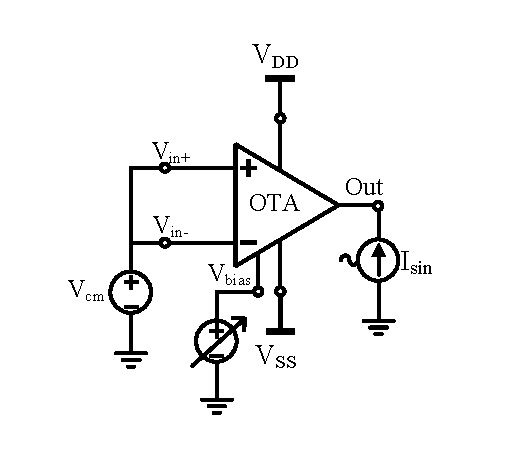
\includegraphics[scale=1]{Figures/Test_Benches/OTA/OTA_Zout.pdf}
\caption{OTA Test setup for calculating Output Impedance}
\label{fig:OTA_TB_ZOUT}
\end{figure}
As discussed in the theory chapter, OTAs generally have high output impedance. And its variation with respect to $V_{bias}$ is tabulated in the Table.\ref{tab:OTA_ZOUT}
\begin{table} [H]
\centering
\begin{tabular}{@{}cccccccc@{}}
\toprule
Vbias (mV)					& 150		& 200			& 300			& 400			& 500			& 600			& 700 \\ \midrule
Output Impedance (k$\Omega$)			& 1.262		& 1.3		& 1.382		& 1.473		& 1.577		& 1.697		& 1.837 \\
\bottomrule
\end{tabular}
\caption{Output Impedance of the OTA}
\label{tab:OTA_ZOUT}
\end{table}

\section{OP AMP Design}
The second stage of the design is the Operational Amplifier. This stage too, like the first stage uses a bipolar power supply of 2.5V and -2.5V. A two-stage Miller compensated op amp is designed and it is used as a Voltage Buffer for the OTA.
\subsection{Schematic}
The schematic of the Miller compensation op amp is as shown in the Figure.\ref{fig:OPAMP_Schematic}. The bias current to the differential pair is provided through the current mirror pair of $M_5$ and $M_8$. The bias current is controlled through the transistor $M_9$ whose gate voltage is provided by the voltage divider formed by the resistors $R_{b1}$ and $R_{b2}$. $C_C$ is the compensation capacitance between the two stages of the amplifier.
\begin{figure} [H]
\centering
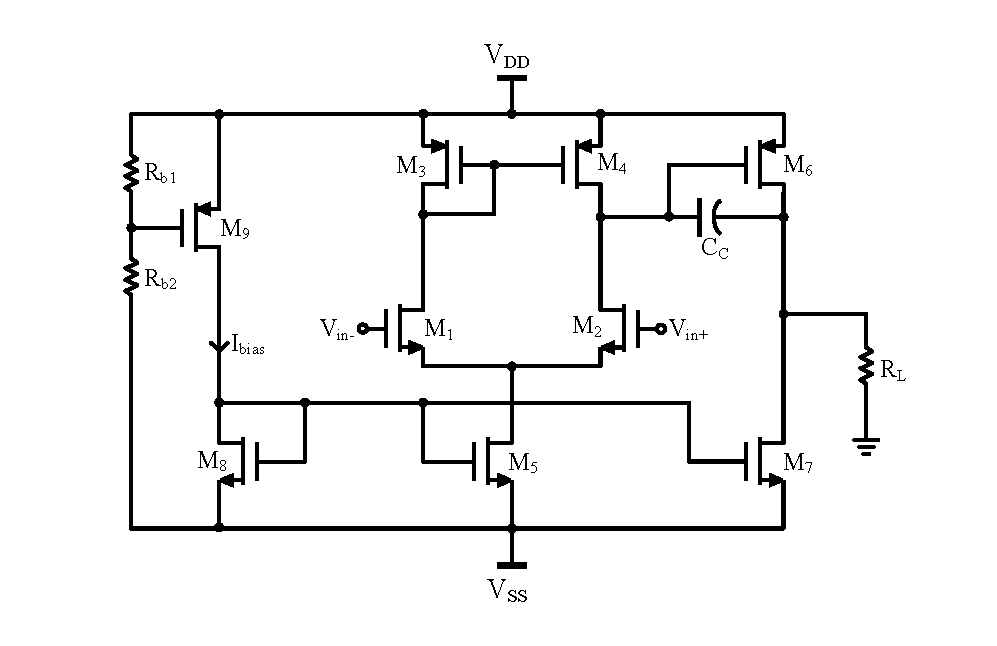
\includegraphics[scale=1]{Figures/Schematics/OPAMP_Vbias.pdf}
\caption{Schematic of the OPAMP Designed}
\label{fig:OPAMP_Schematic}
\end{figure}

The dimensions of the transistors are tabulated in Table.\ref{tab:OPAMP_dimensions}. One can easily recognize that the transistors at the output are large. This is designed so to make sure the op amp provides a very high current and thereby avoiding a common collector amplifier at the output of the op amp to amplify the output current. The compensation capacitance value is 50fF.

\begin{table} [H]
\centering
\begin{tabular}{@{}cccc@{}}
\toprule
Transistor			& Width				& Length			& Multiplier \\ \midrule
M1					& 5u				& 500n				& 2			\\
M2					& 5u				& 500n				& 2			\\ 
M3					& 30u				& 500n				& 1			\\
M4					& 30u				& 500n				& 1			\\ 
M5					& 2u				& 500n				& 1			\\
M6					& 85u				& 500n				& 55		\\ 
M7					& 50u				& 500n				& 48		\\
M8					& 2u				& 500n				& 1			\\ 
M9					& 700n				& 500n				& 1			\\
\bottomrule
\end{tabular}
\caption{Dimensions of the Transistors of the designed OPAMP}
\label{tab:OPAMP_dimensions}
\end{table}

\subsection{Test Setup}
In the following subsections, the typical parameters of an op amp are simulated and analysed.
\subsubsection{DC Analysis}

Input Common Mode Range or ICMR of an operational amplifier is the range of the common mode input voltage over which the amplifier behaves as a linear amplifier fir differential input signals. In simpler words, the ICMR is defined by the input voltages at which all the transistors remain in saturation. Figure.\ref{fig:OPAMP_TB_ICMR} shows the test setup to measure the ICMR of the op amp designed.
\begin{figure} [H]
\centering
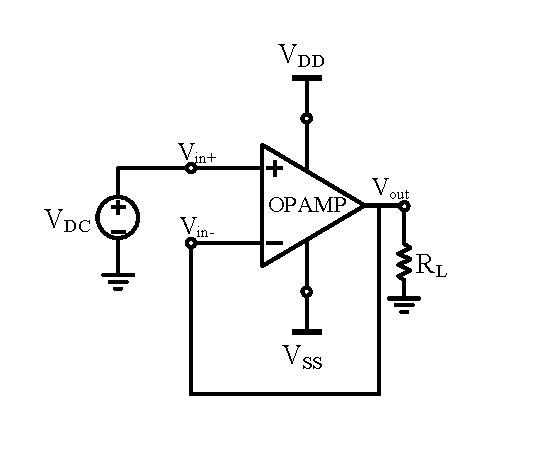
\includegraphics[scale=1]{Figures/Test_Benches/OPAMP/OPAMP_ICMR.pdf}
\caption{OPAMP Test setup for calculating ICMR}
\label{fig:OPAMP_TB_ICMR}
\end{figure}

The transistors which impact the ICMR are $M_3, M_4$ and $M_5$. These transistors were designed in such a way that the op amp ICMR lies between -2V and 2V. The DC input voltage at the non-inverting terminal is swept in the range of $V_{DD}$ and $V_{SS}$, i.e., 2.5V to -2.5V. The plot of DC output voltage for a varying DC input voltage is as shown inFigure.\ref{fig:OPAMP_ICMR}. It can be noted that the minimum value of the ICMR is -2.19V and the maximum value of the ICMR is  2.089V.

\begin{figure} [H]
\centering
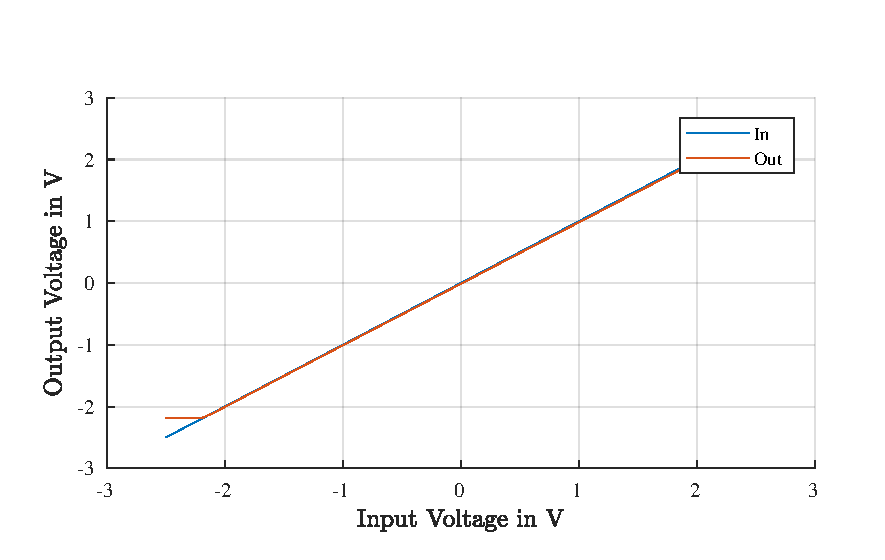
\includegraphics[scale=1]{Figures/Plots/OPAMP_ICMR.pdf}
\caption{OPAMP Plot of ICMR vs Vin}
\label{fig:OPAMP_ICMR}
\end{figure}

The output voltage swing is the range of voltage that an opamp can physically provide at its output. On the same lines as ICMR but without feedback, the output voltage swing is measured and plotted with respect to the input voltage. And the output voltage ranges from -2.19 to 2.323. The plot is as shown in Figure.\ref{fig:OPAMP_Swing}.

\begin{figure} [H]
\centering
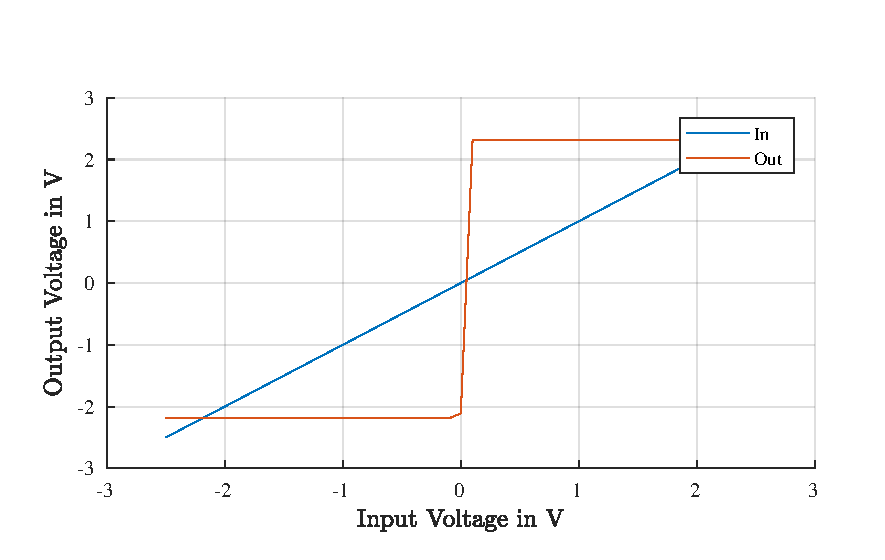
\includegraphics[scale=1]{Figures/Plots/OPAMP_OutSwing.pdf}
\caption{OPAMP Plot of Output Voltage Swing vs Vin}
\label{fig:OPAMP_Swing}
\end{figure}

\subsubsection{AC Analysis}
The open loop gain and the gain bandwidth product are inarguably the most important parameters of an operational amplifier. Before the op amp was actually designed, these parameters were simulated with the help of an ideal op amp from the ahdlLib in Cadence. In order to have a stable system, i.e., an OTA with an OP AMP buffer in a cascade configuration, it is necessary to have the dominant poles far from each other. So that is the reason for the OTA to have a high bandwidth and correspondingly the OP AMP bandwidth can be adjusted so as to reach the specification and also to have a stable system.

The test bench used to measure these parameters is as shown in Figure.\ref{fig:OPAMP_TB_ACDC}. The op amp is configured in an open loop. The DC biasing to the differential transistor pair is provided by the output of the OTA, which is centred around 0V. 

$V_{DD}$ = 2.5V; $V_{SS}$ = -2.5V; $V_{ac} magnitude $ = 1 V; $R_L$ = 50$\Omega$.

\begin{figure} [H]
\centering
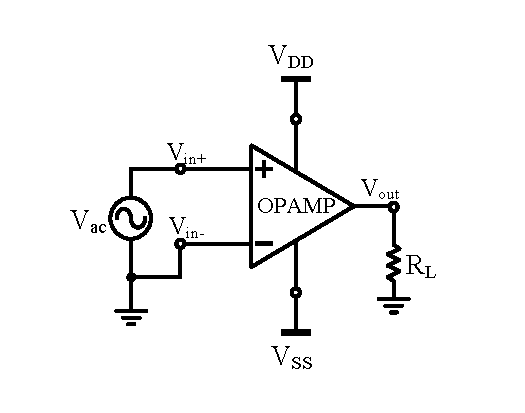
\includegraphics[scale=1]{Figures/Test_Benches/OPAMP/OPAMP_ACDC.pdf}
\caption{OPAMP Test setup for AC, DC and Noise Analysis}
\label{fig:OPAMP_TB_ACDC}
\end{figure}

The plot of the open loop gain and the phase of the op amp is as shown in the Figure.\ref{fig:OPAMP_gain_pm_gbw}. The open loop gain of the op amp is 30.8dB. The gain bandwidth product is 6.2MHz and correspondingly the phase margin is $76.79^0$.

\begin{figure} [H]
\centering
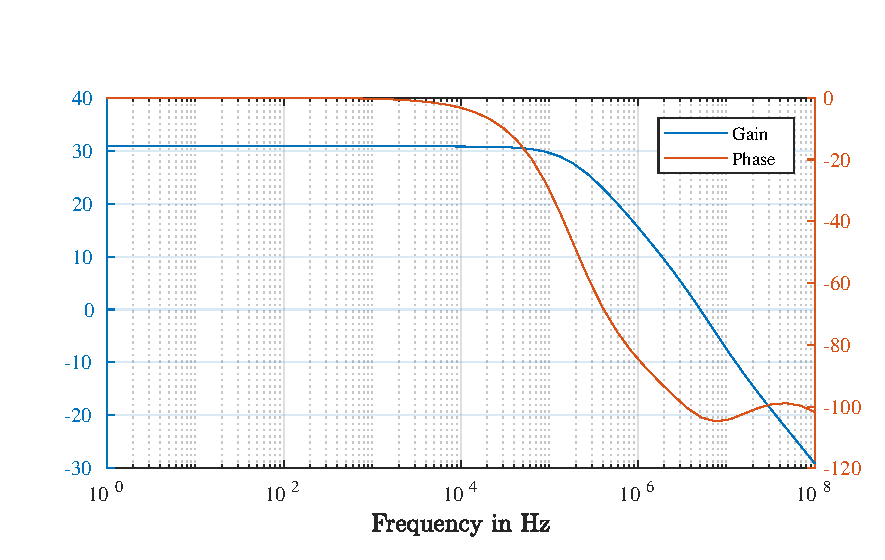
\includegraphics[scale=1]{Figures/Plots/OPAMP_Gain_PM.pdf}
\caption{OPAMP Plot of Gain and Phase vs Frequency}
\label{fig:OPAMP_gain_pm_gbw}
\end{figure}

The PSRR of the OTA in the first stage was in the range of $nA/V$ and hence neglibigle. However, the op amp designed exhibits a relatively high value of PSRR. This is due to the bulky transistors at the output stage. The test bench to measure the PSRR of the op amp is as shown in the Figure.\ref{fig:OPAMP_TB_PSRR}. The one on the left is used to measure PSRR for a change in $V_{DD}$. And similarly, the one on the right side is used to measure PSRR for a change in $V_{SS}$.

$V_{DD}$ = 2.5V; $V_{SS}$ = -2.5V; $V_{ac} magnitude $ = 1 V; $R_L$ = 50$\Omega$.
\begin{figure} [H]
\centering
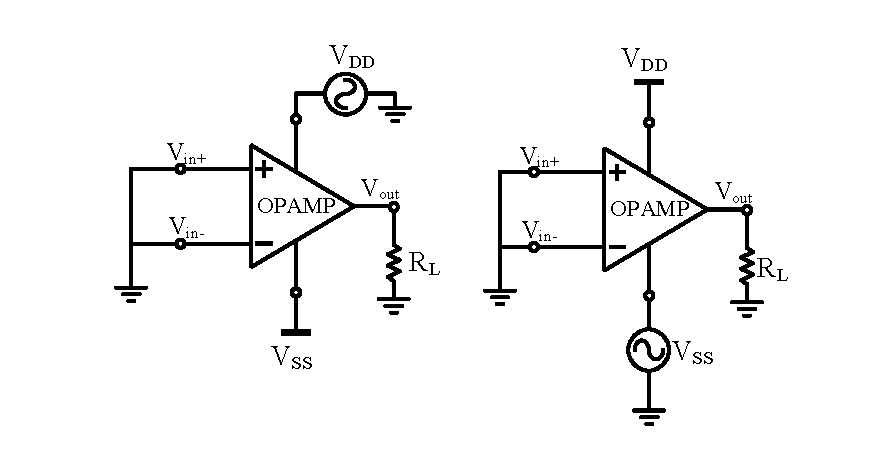
\includegraphics[scale=1]{Figures/Test_Benches/OPAMP/OPAMP_PSRR.pdf}
\caption{Test setup for calculating PSRR}
\label{fig:OPAMP_TB_PSRR}
\end{figure}

The PSRR ($V_{DD}$) of the op amp is 30.96 uA/V, and PSRR ($V_{SS}$) is 130.96 uA/V. In the next chapter, it is seen that the assymetry in the two PSRR values doesn't affect the PSRR of the whole system.

The test bench to calculate the input impedance follows a similar concept to that of the OTA. i.e., a unitz current source is connected to the non-inverting terminal of the op amp and the voltage at that terminal is measured which in turn is the magnitude of the input impedance of the op amp.

$V_{DD}$ = 2.5V; $V_{SS}$ = -2.5V; $I_{sin} magnitude $ = 1A; $R_L$ = 50$\Omega$.
\begin{figure} [H]
\centering
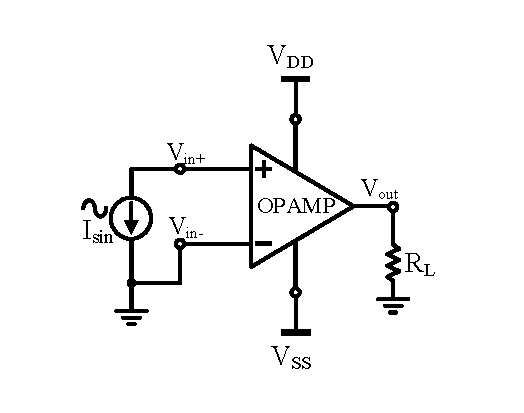
\includegraphics[scale=1]{Figures/Test_Benches/OPAMP/OPAMP_Zin.pdf}
\caption{Test setup for calculating Input Impedance}
\label{fig:OPAMP_TB_ZIN}
\end{figure}

To have a stable system, it is important that input impedance of the second stage is higher than the output impedance of the first stage. Given that the output impedance of the OTA is generally high, the input impedance of the op amp becomes a very important parameter. And th input impedance is found to be 9.04M$\Omega$.

On the same lines, the test bench to measure the output impedance of the op amp is as shown in Figure.\ref{fig:OPAMP_TB_ZOUT}. The resistive load is replaced by a current source with unity magnitude. And hence the voltage at the output will be the magnitude of the output impedance of th op amp.


$V_{DD}$ = 2.5V; $V_{SS}$ = -2.5V; $I_{sin} magnitude $ = 1A.
\begin{figure} [H]
\centering
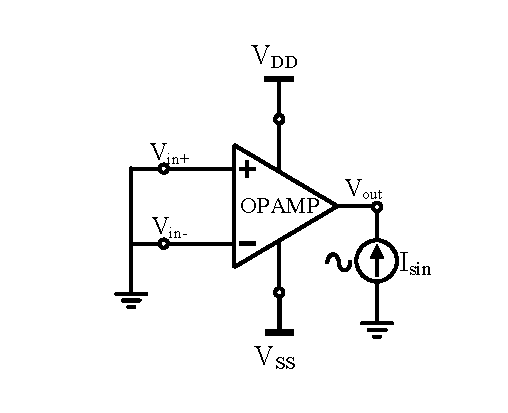
\includegraphics[scale=1]{Figures/Test_Benches/OPAMP/OPAMP_Zout.pdf}
\caption{Test setup for calculating Output Impedance}
\label{fig:OPAMP_TB_ZOUT}
\end{figure}

Op amps are known to have zero or very low output impedance. Along with this theoretical fact, the op amp in this work is designed to retrieve very high currents, so it is expected to have a very low output impedance. The value of the output impedance is observed to be 4.167$\Omega$.


\subsubsection{Transient Analysis}
The test bench to perform the transient analysis is as shown in the Figure.\ref{fig:OPAMP_TB_Sine}. The op amp is connected in a negative feedback configuration so as to analyse its behavior as a voltage buffer.

$V_{DD}$ = 2.5V; $V_{SS}$ = -2.5V; $V_{sin} amplitude $ = 1.5V; $frequency$ = 1MHz; $R_L$ = 50$\Omega$.
\begin{figure} [H]
\centering
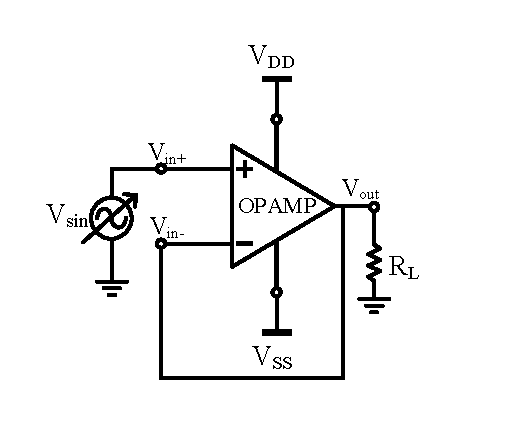
\includegraphics[scale=1]{Figures/Test_Benches/OPAMP/OPAMP_Sine.pdf}
\caption{Test setup for Transient Analysis - Sine Wave Input}
\label{fig:OPAMP_TB_Sine}
\end{figure}

The of input voltage and output voltage with respect to time is as shown in the Figure.\ref{fig:OPAMP_Vout}. The output follows the input only with a very small delay.

\begin{figure} [H]
\centering
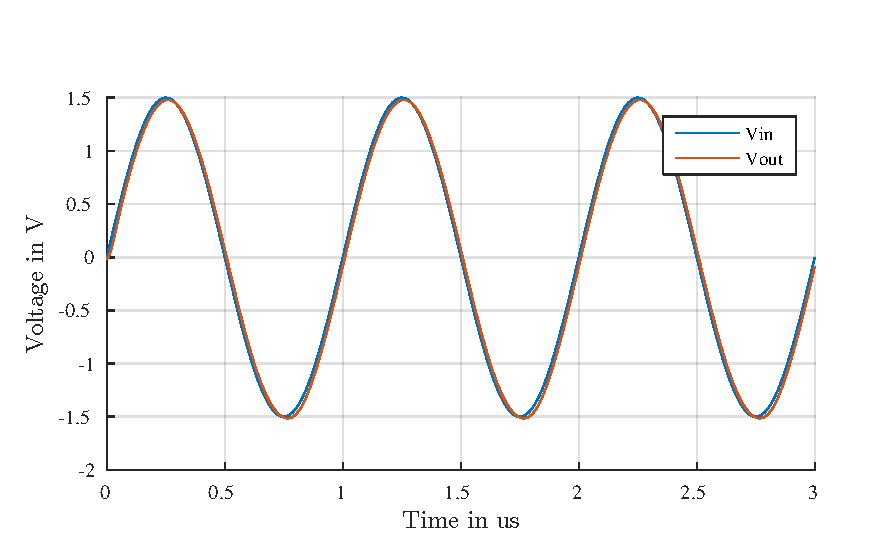
\includegraphics[scale=1]{Figures/Plots/OPAMP_Buffer.pdf}
\caption{OPAMP Plot of Output Voltage vs time}
\label{fig:OPAMP_Vout}
\end{figure}

The output current of the op amp is effectively the current flowing through the load resistor $R_L$. The plot of current versus time is as shown in the Figure.\ref{fig:OPAMP_Iout}. The current is $180^0$ out of phase with the voltage and it ranges from -30mA to 30mA for a 50$\Omega$ load and 3V peak to peak input voltage. 

\begin{figure} [H]
\centering
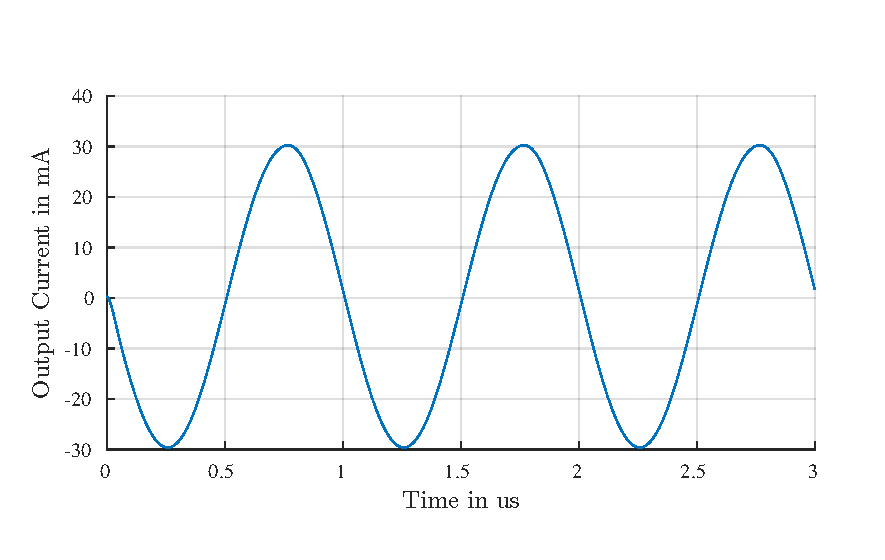
\includegraphics[scale=1]{Figures/Plots/OPAMP_Iout.pdf}
\caption{OPAMP Plot of Ourput Current vs time}
\label{fig:OPAMP_Iout}
\end{figure}

The only change from the previous test bench to this is that we need to replace the sinusoidal source by a pulse input source.
\begin{figure} [H]
\centering
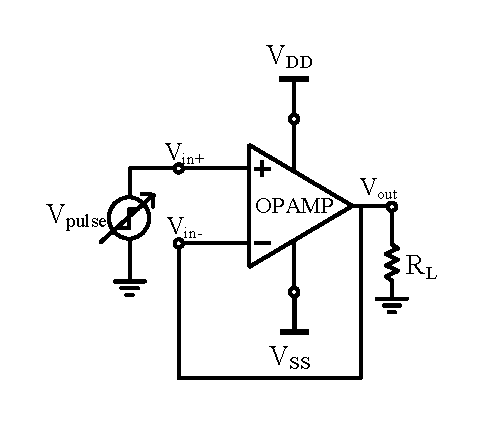
\includegraphics[scale=1]{Figures/Test_Benches/OPAMP/OPAMP_Slew.pdf}
\caption{Test setup for Transient Analysis - Square Wave Input}
\label{fig:OPAMP_TB_Slew}
\end{figure}

The values of all the parameters of the op amp discussed so far have been tabulated in Table.\ref{tab:OPAMP_Results}
\begin{table} [H]
\centering
\begin{tabular}{@{}cc@{}}
\toprule
Parameter					& Value				\\ \midrule
Open Loop Gain				& 30.8 dB			\\
Gain Bandwidth Product		& 6.2 MHz			\\
Phase Margin				& 76.79				\\
ICMR (min)					& -2.19 V			\\
ICMR (max)					& 2.089 V			\\
Output Current (max)		& -29.6 mA			\\
Output Current (min)		& 30.28 mA			\\
Output Voltage Swing		& -2.19 .. 2.323 	\\
Slew Rate					& 10 V/us			\\
PSRR (VDD)					& 30.96 uA/V		\\
PSRR (VSS)					& 138.8 uA/V		\\
Input Impedance				& 9.04 MOhms		\\
Output Impedance			& 4.167 Ohms		\\
\bottomrule
\end{tabular}
\caption{Simlation Results of the OPAMP}
\label{tab:OPAMP_Results}
\end{table}

\section{The Complete Design}
The block diagram of the two stage design with an OTA and an OP AMP is as shown in Figure.\ref{fig:System_Block_Diagram}. The other end of the capacitor of the first stage is connected to the negative power supply instead of ground since we have only two levels in the IC (-2.5V and 2.5V). Both the stages use the same power supply. The output of the OTA is directly connected to the non-inverting terminal of the OP AMP without any DC isolation via a coupling capacitor.

\begin{figure} [H]
\centering
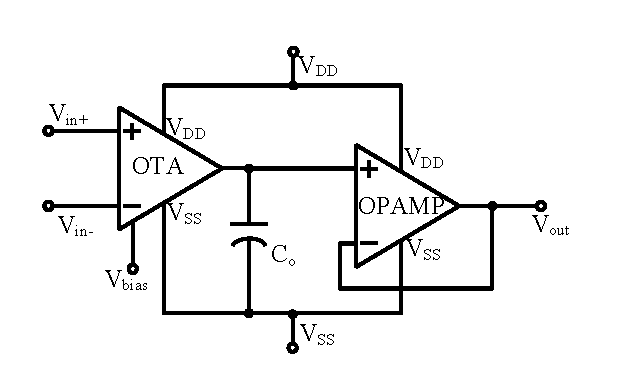
\includegraphics[scale=1]{Figures/System_Level/System_Overview.pdf}
\caption{Block Diagram of the Overall System}
\label{fig:System_Block_Diagram}
\end{figure}

The schematic symbol for the overall system is as indicated in Figure.\ref{fig:System_Symbol}. The block diagram of the system is drawn inside to get an understanding of the configuration.

\begin{figure} [H]
\centering
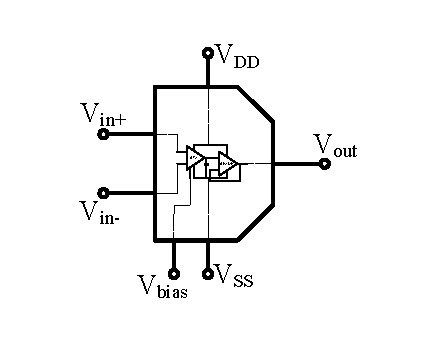
\includegraphics[scale=1]{Figures/System_Level/System_Symbol.pdf}
\caption{Schematic Symbol for the Overall System}
\label{fig:System_Symbol}
\end{figure}

\subsection{Schematic}
The transistor level schematic of the overall system is as shown in the Figure.\ref{fig:System_Schematic}. The upper portion of the schematic is the OTA and the bottom portion is the OP AMP. Note the feedback connection of the OP AMP and the connection between the OTA and the OP AMP. To summarize the physical aspects of the system, there are 3 input terminals, 2 power supply levels and 1 ouput pin.
 
\begin{figure} [H]
\centering
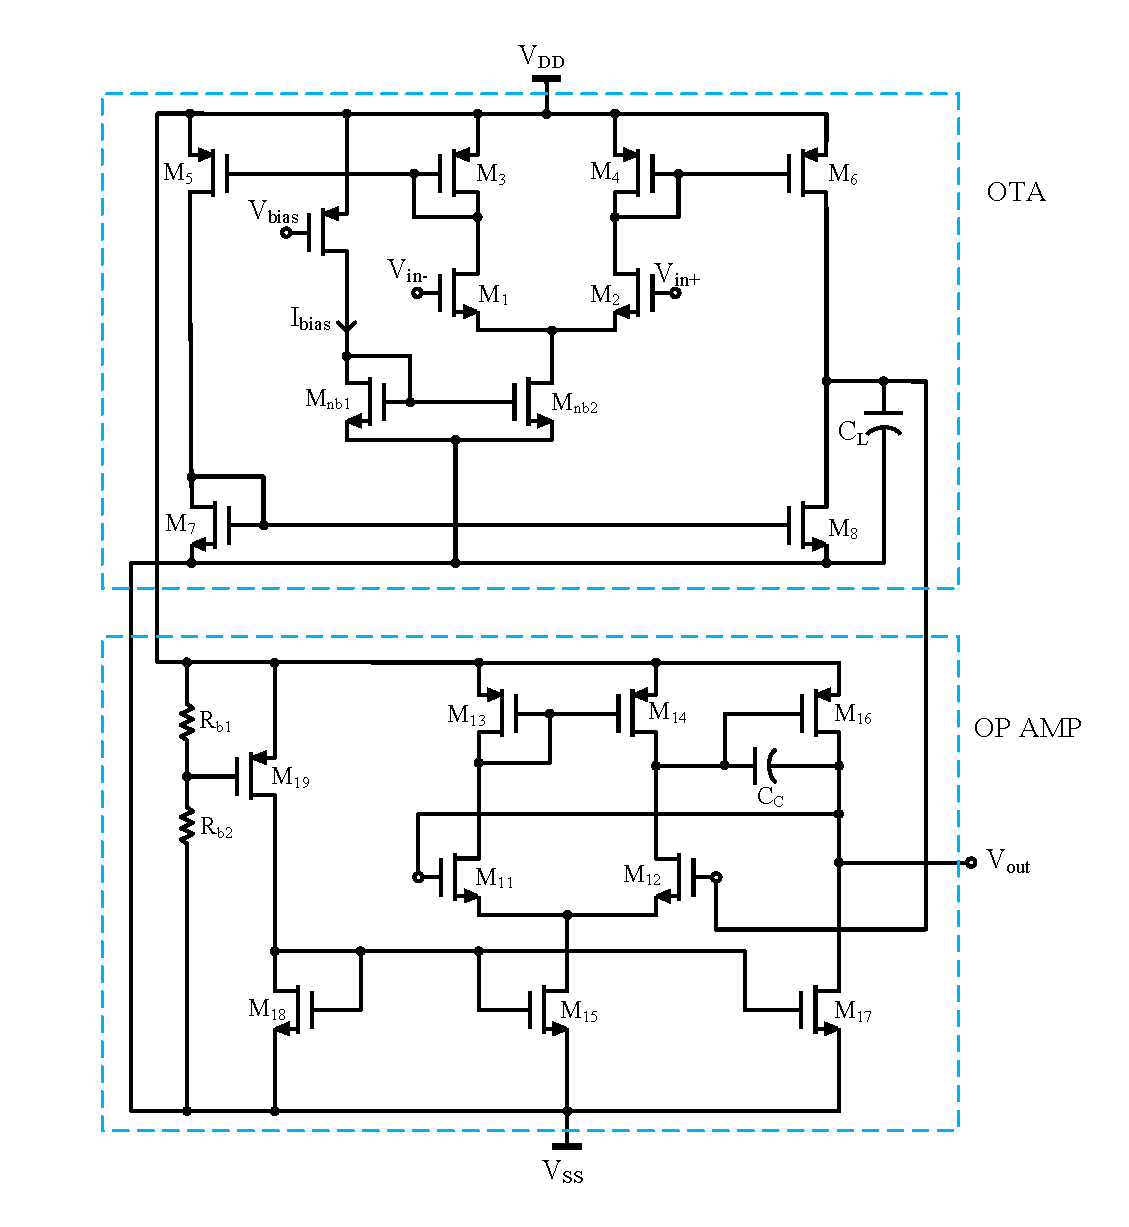
\includegraphics[scale=1]{Figures/Schematics/OTA_OPAMP_Schematic.pdf}
\caption{Schematic Diagram for the Overall System}
\label{fig:System_Schematic}
\end{figure}
